%!TEX root = ../../../report.tex
\section{Joints design} % (fold)
\label{sec:joints}
Following the idea of mimicking the human lower-body structure it was decided to implement three actuated rotational joints per leg although some research was conducted on the use of passive ankles as in \cite{dacbot1}, \cite{phides} or \cite{mabel}.
However, the results introduced in \cite{grimmer} from their analysis of joint actuation for prosthetics limbs proved the importance of the actuation in the ankles for running.

The design of the joints entailed the addressing of three main areas

\begin{itemize}
  \item Actuator model
  \item Transmission system
  \item Implementation of dedicated compliance
\end{itemize}

\subsection{Actuators} % (fold)
\label{sub:actuators}
In humans, the actuation of the joints is mostly provided by pairs of agonist-antagonist skeletal muscles linked to the bones through the tendons \cite{anatomy}.
The activation-inhibition of these muscles produce a lever effect on the bones that leads to its control and motion by modifying the angle between two consecutive limbs.
To achieve the same kind of motion control, the implementation of a similar system through electric linear actuators was considered.
However, the time constraints, their price and their complexity led to discard them and select conventional electric motors.
The selected motor model will have to be able to provide a sufficient torque to generate the desired forces at the end of the link, following equation \ref{eq:torque}.

\begin{equation}
\label{eq:torque}
  \tau = r \times F
\end{equation}

This equation could be sufficient to compute the torque required by the load for a motor application of leverage. 
However, an study of each joint separately would not provide an accurate enough solution due to the configuration of the legs, making necessary an study of the actuation as for a kinematic chain.
The analysis of the actuators requirements is to be found in \ref{cha:mathematical_model}.

% subsection actuators (end)

\subsection{Torque transmission} % (fold)
\label{sub:transmission}
As introduced in \ref{sub:moments_of_inertia}, the reduction of the moments of inertia in the limbs in order to minimize the torque requirements for motion was set as a priority.
This led to the study of methods to displace the CoM of the limbs as close to their joints axes as possible, thus reducing their inertias.
The solution was to place the actuators, the heaviest components of the design, as close to the upper part of the frame as possible, which would also result in the allocation of the CoM of the frame upper in the sagital plane.
An schematic example of this idea can be seen in the Figures in \ref{fig:compliance} for the ankle actuation, where the motor has been placed under the knee axis. 
The same principle has been applied to the knee actuation, as can be seen in the final implementation. 
For the hip, however, it was not necessary to install a transmission system, but a gear mechanism whose justification is to be found in \ref{cha:mathematical_model}.

Due to the new arrangement, a powertrain was required to transmit the torque to the joints.
It was decided to implement a system of 2 pulleys + belt due to its simplicity and optimal capabilities for the project requirements.
The goal of this mechanism is only the transmission of power, without any further adjustment of angular speed-torque ratios.
The calculations to find the optimal dimensions of the system are contained in \ref{sub:pulleys_and_belts}.
The pitfall of this implementation, however, is the introduction of delays in the motion transmission and the natural loss of accuracy arisen from the backlash associated to the use of pulleys.
Modeling these uncertainties for a classic locomotion controller based on the motion equations is proved a complex task. 
However it was assumed here that the ANN controllers that would drive the RuBi platform would be able to adapt to them without a model of the robot.

% subsection transmission (end)

\subsection{Joints compliance} % (fold)
\label{sub:compliance}
The advantages of the incorporation of compliance in legged locomotion have been broadly demonstrated in \cite{compliance_thesis} and \cite{grimmer}.
Compliance in running and walking gait generation is used to reduce actuators requirements through the minimization energy consumption.
Furthermore, it helps isolate the joints of the structure from the impact forces created during the landing phase, reinforcing the mechanical capabilities of the structure.
This section deals with the study and selection of the configuration of the elastic actuators and their distribution in the legs.
The numerical estimation of the actual springs to be used in the robot can be seen in \ref{sec_springs}.

\subsubsection{Elastic actuators configuration} % (fold)
\label{ssub:elastic_actuator_configuration}
Several elastic actuator configurations have been defined in the literature, from which four ones have been studied here and are shown in Figure \ref{fig:series_actuators}.
The most detailed analysis of the influence of each of these configurations in energy storage and power consumption in human locomotion has been found in \cite{grimmer}.
In that paper, the normalized power requirements with the different configurations have been tested for a range of gaits, easing the process of finding the optimal configuration and its parameters for a specific gait and velocity.
However, the fact that RuBi is not being designed for a specific gait or velocity, but as a platform to study the transition between gaits and velocity adaption, makes the estimation of the best configuration an under-determined problem.
This reasoning led to the implementation of a new feature in RuBi, the full reconfigurability of the compliance in its actuators.
This capability allows for the possibility of studying in the real platform the influence of the elastic actuators on its performance and its control, giving RuBi a whole new set of uses.

\begin{figure}[h]
\label{fig:series_actuators}
\centering
  \begin{subfigure}{.15\textwidth}
    %\centering
    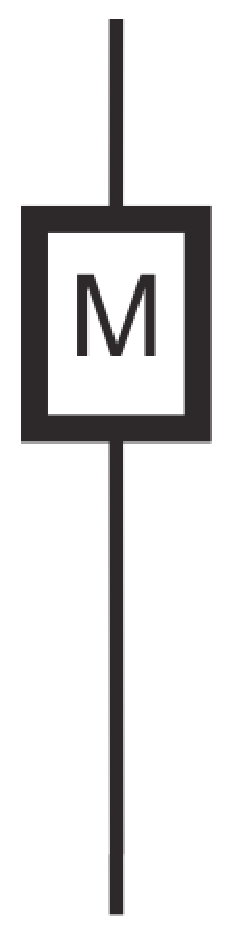
\includegraphics[width=0.63\linewidth]{figures/ddact.pdf}
    \caption{DD}
    \label{fig:series_pulley}
  \end{subfigure}
  \begin{subfigure}{.15\textwidth}
    %\centering
    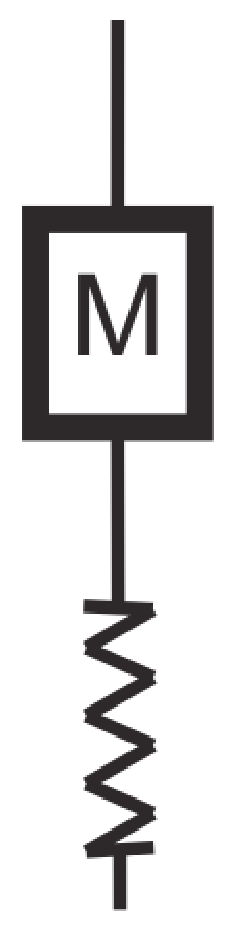
\includegraphics[width=0.63\linewidth]{figures/SEAact.pdf}
    \caption{SEA}
    \label{fig:series_rotational}
  \end{subfigure}
  \begin{subfigure}{.15\textwidth}
    %\centering
    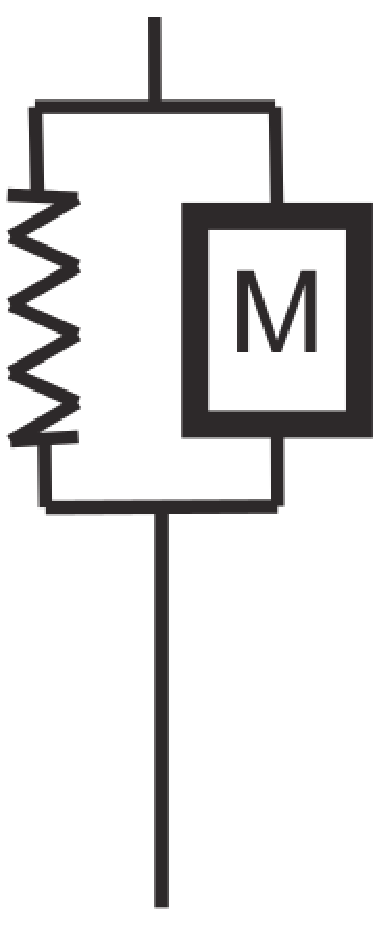
\includegraphics[width=\linewidth]{figures/PEAact.pdf}
    \caption{PEA}
    \label{fig:series_direct_i}
  \end{subfigure}
  \begin{subfigure}{.15\textwidth}
    %\centering
    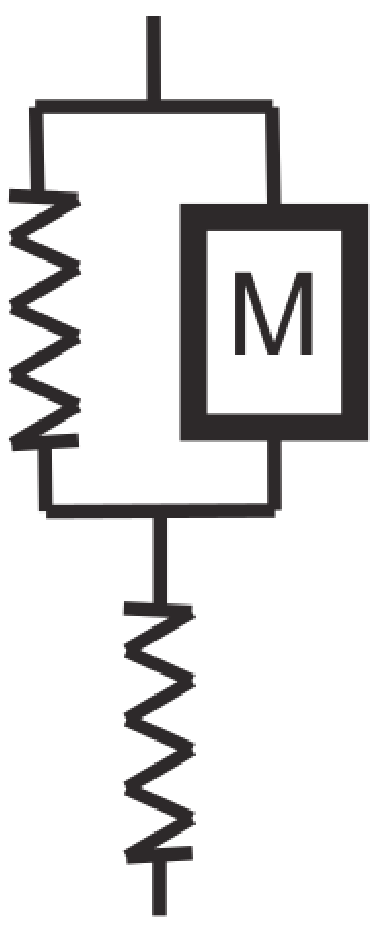
\includegraphics[width=\linewidth]{figures/SEA+PEAact.pdf}
    \caption{SEA+PEA}
    \label{fig:series_direct_ii}
  \end{subfigure}
  \caption{Four configurations for elastic actuators as from \cite{grimmer}}
\end{figure}  


%Flexible vs stiff drive train
%Power peak and average consumption comparisons --> energy storage 
%Protection against impact forces on landing phase
% subsubsection elastic_actuator_configuration (end)

\subsubsection{Compliance distribution and implementation} % (fold)
\label{ssub:compliance_distribution_and_possible_configurations}
The results in \cite{grimmer} demonstrate that the implementation of compliance in any of its variants in knees and ankles influences notably the peak power and energy requirements both for walking and running.
They also seem to prove that the contribution to the reduction of energy consumption and power requirements of the hip is neglectable.
These findings have been used to justify the implementation of elastic actuators in knees and ankles, but not in the hip joints, actuated through direct transmission.

Several models from literature have been subject to a comparative analysis for their use in RuBi, being the main ones shown in Figure \ref{fig:compliance} for the ankle actuation (equivalent for the knees).
These schematics depict the three major design choices made so far, summarized in \ref{list:design_criterias}.
A short summary of the conclusions reached by these studies is introduced below.

\begin{itemize}
\label{list:design_criterias}
  \item Reduction of limbs inertias by placing the actuators up on the links.
  \item Use of transmission to solve the transfer of power motor-joint.
  \item Introduction of compliance through the use of springs.
\end{itemize}

\paragraph{SEA 1 and 2} % (fold)
\label{par:sea_1_2}
\ref{fig:series1} depicts an unidirectional SEA that has to be implemented together with a counterpart, which could be a passive spring or another actuator.
In that case the actuator task would only be the retraction of the foot to reduce its angle with respect to the lower leg, while the passive spring function would imitate the calf muscle.
This approach would be closer to the real functioning of the muscles in the legs, as explained in \ref{sec:bipedal_walking_and_running_gaits}.
However this configuration was discarded due to the complexity in the realization of a correct mapping between the angular displacement of the motor pulley and the ankle joint.

The configuration in Figure \ref{fig:series2} was found in \cite{biobiped}.
It solves the problem found for \ref{par:sea_1} changing the configuration of the motor and introducing a fixed pulley.
The influence of the relationship between $L_{B}$ and $L_{A}$ in the ratio between motor and joint torques was studies for this configuration in order to find the optimal dimensions.
However, this solution was discarded in favor of the current one, which demonstrated to be simpler to implement.
% paragraph sea_1_2 (end)

\paragraph{SEA 3} % (fold)
\label{par:sea_3}
The spring configuration in \ref{fig:series3} was found in \cite{grimmer} for a prosthetic ankle design (meaning that the configuration should be adapted for the knee).
It was just used as a study case and source of ideas. 
% paragraph sea_3 (end)

\paragraph{SEA 4} % (fold)
\label{par:sea_4}
The configuration in \ref{fig:series4} was also found in \cite{biobiped} and is known as bidirectional SEA.
It was considered the most optimal to mimic the human musculature on the legs and its implementation through springs attached to the belts or with elastic bands (bungee cords) like the utilized in \cite{imperial_college} was object of analysis.
% paragraph sea_4 (end)

\paragraph{SEA 5} % (fold)
\label{par:sea_5}
The configuration called SEA 5 and shown in Figure \ref{fig:series5} was the selected one.
The original idea was taken from \cite{phides} but has been modified to ease its construction and provide more robustness to the final design.
In \cite{phides} this elastic transmission is implemented with torsion bars for the joints axes, while RuBi uses torsion springs placed around more resistant axis to transmit the motion.
% paragraph sea_5 (end)

\begin{figure}[hb!]
\label{fig:compliance}
  \begin{subfigure}{.19\textwidth}
    \centering
    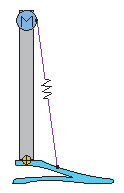
\includegraphics[width=\linewidth]{figures/illustration_serial_direct_i.pdf}
    \caption{SEA 1}
    \label{fig:series1}
  \end{subfigure}
  \begin{subfigure}{.19\textwidth}
    \centering
    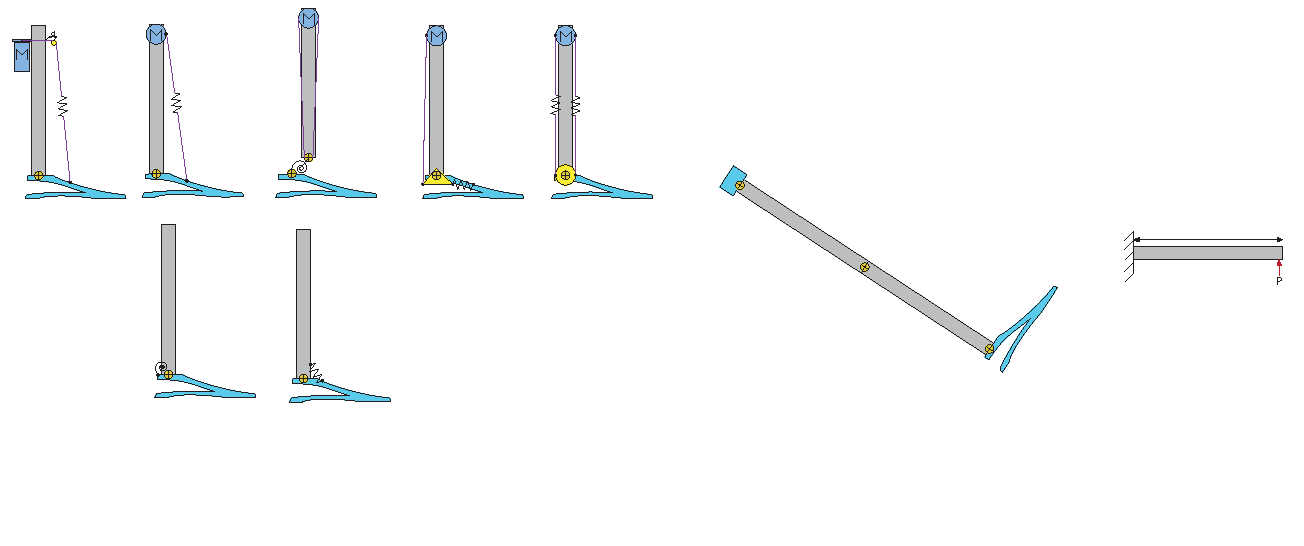
\includegraphics[width=\linewidth]{figures/illustration_serial_pulley.pdf}
    \caption{SEA 2}
    \label{fig:series2}
  \end{subfigure}
  \begin{subfigure}{.19\textwidth}
    \centering
    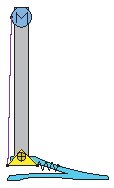
\includegraphics[width=\linewidth]{figures/illustration_serial_direct_ii.pdf}
    \caption{SEA 3}
    \label{fig:series3}
  \end{subfigure}
  \begin{subfigure}{.19\textwidth}
    \centering
    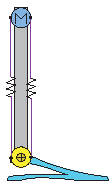
\includegraphics[width=\linewidth]{figures/illustration_serial_elastic_band.pdf}
    \caption{SEA 4}
    \label{fig:series4}
  \end{subfigure}
  \begin{subfigure}{.19\textwidth}
    \centering
    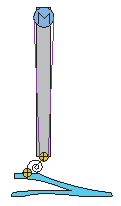
\includegraphics[width=\linewidth]{figures/illustration_serial_rotational.pdf}
    \caption{SEA 5}
    \label{fig:series5}
  \end{subfigure}
\end{figure}  
% subsubsection compliance_distribution_and_possible_configurations (end)

% subsection compliance (end)

% section joints (end)